\section{Dépendances fonctionnelles}

%\subsection{Définitions}
\begin{frame}
  \frametitle{Dépendances fonctionnelles}
  \begin{itemize}
    \item Méthode pour établir efficacement un modèle entités-associations bien normalisé:
      \begin{enumerate}
        \item Étudier les dépendances fonctionnelles
        \item Obtention du graphe de couverture minimale
        \item Traduction du graphe en modèle
      \end{enumerate}
    \item Traditionnellement employé pour normaliser des modèles relationnels
  \end{itemize}
\end{frame}

\begin{frame}
  \frametitle{Définition}
  \begin{itemize}
    \item Un attribut $Y$ dépend fonctionnellement d'un attribut $X$ si et seulement si une valeur de $X$ induit une
      unique valeur de $Y$
    \item On note une dépendance fonctionnelle par une flèche simple : $$X \ra Y$$
  \end{itemize}
\end{frame}

\begin{frame}
  \frametitle{Transitivité}
  \begin{itemize}
    \item Une dépendance fonctionnelle est transitive : $$\text{si } X \ra Y \text{ et } Y \ra Z \text{ alors } X \ra Z$$
    \item Exemple:\\
      si \emph{numéro commande} $\ra$ \emph{numéro client} $\ra$ \emph{nom client}\\
      alors \emph{numéro commande} $\ra$ \emph{nom client}
    \item Deux types de dépendances fonctionnelles :
      \begin{itemize}
        \item directe: \emph{numéro commande} $\ra$ \emph{numéro client}
        \item transitive: \emph{numéro commande} $\ra$ \emph{nom client}
      \end{itemize}
  \end{itemize}
\end{frame}

\begin{frame}
  \frametitle{Dépendances fonctionnelles non élémentaires}
  \begin{itemize}
    \item Dépendance fonctionnelles non élémentaire :\\
      Un attribut $Y$ a une dépendance fonctionnelle qui repose sur la conjonction de plusieurs
      attributs
    \item On note une dépendance fonctionnelle non élémentaire par une flèche unique avec plusieurs points
      d'entrée (regroupés autour d'un cercle)
  \end{itemize}
  \begin{center}
    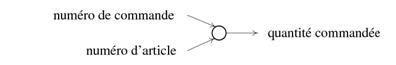
\includegraphics[width=0.9\linewidth]{dependance_fonctionnelle_non_elementaire.jpg}
  \end{center}
  \begin{itemize}
  \item Dans l'exemple, dépendance fonctionnelle à la fois non élémentaire et directe
  \end{itemize}
\end{frame}

\begin{frame}
  \frametitle{Graphe de couverture minimale}
  \begin{itemize}
    \item Graphe de couverture minimale :\\
      Réseau obtenu en représentant tous les attributs et toutes les dépendances fonctionnelles directes entre
      ces derniers
  \end{itemize}
  \begin{center}
    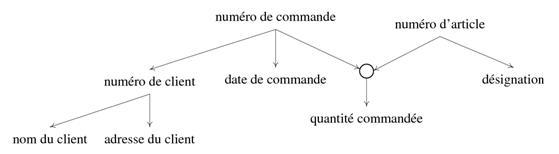
\includegraphics[width=0.9\linewidth]{graphe_couverture_minimale.jpg}
  \end{center}
\end{frame}

%\subsection{Méthodologie}
\begin{frame}
  \frametitle{Méthodologies}
  \begin{itemize}
    \item Nous avons vu à la fin de la section \og Modèle conceptuel \fg\ une méthodologie pour obtenir un
      modèle conceptuel de donnée
    \item Nous allons maintenant voir une méthodologie à partir de l'étude des dépendances fonctionnelles
      directes
  \end{itemize}
\end{frame}

\begin{frame}
  \frametitle{Méthodologie classique}
  \begin{enumerate}
    \item Identifier les entités en présence
    \item Lister leurs attributs
    \item Ajouter les identifiants
    \item Établir les associations binaires entre les entités
    \item Lister leurs attributs
    \item Calculer les cardinalités
    \item Vérifier les règles de normalisation, en particulier:
      \begin{itemize}
        \item Normalisation des entités (associations non binaires, etc.)
        \item Normalisation des associations et des attributs
        \item Troisième forme normale de Boyce-Codd
      \end{itemize}
    \item Effectuer les corrections nécessaires
  \end{enumerate}
\end{frame}

\begin{frame}
  \frametitle{Traduction à partir des dépendances fonctionnelles}
  \begin{itemize}
    \item Plusieurs étapes pour passer du graphe de couverture minimale à un schéma entités-associations normalisé
  \end{itemize}
  \begin{center}
    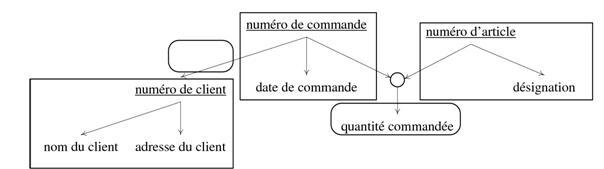
\includegraphics[width=0.9\linewidth]{graphe_identifie_5.jpg}
  \end{center}
\end{frame}

\begin{frame}
  \frametitle{Étapes de traduction (1)}
  \begin{center}
    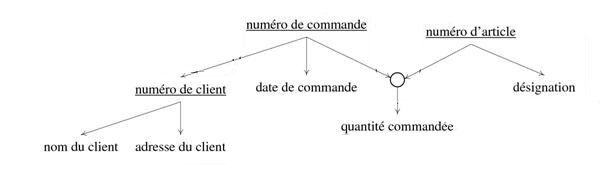
\includegraphics[width=0.9\linewidth]{graphe_identifie_1.jpg}
  \end{center}
  \begin{itemize}
    \item Étape 1 : repérer et souligner les identifiants
  \end{itemize}
\end{frame}

\begin{frame}
  \frametitle{Étapes de traduction (2)}
  \begin{center}
    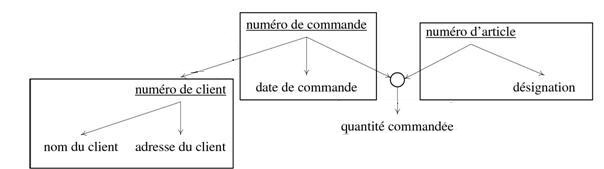
\includegraphics[width=0.9\linewidth]{graphe_identifie_2.jpg}
  \end{center}
  \begin{itemize}
    \item Étape 2 : tous les attributs non identifiant qui dépendent directement d'un identifiant et d'un
      seul, forment (avec l'identifiant) une entité
  \end{itemize}
\end{frame}

\begin{frame}
  \frametitle{Étapes de traduction (3)}
  \begin{center}
    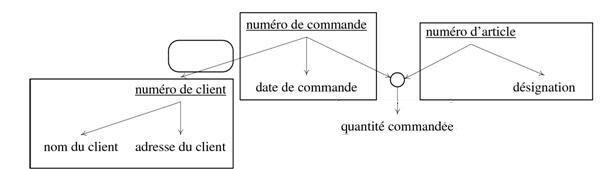
\includegraphics[width=0.9\linewidth]{graphe_identifie_3.jpg}
  \end{center}
  \begin{itemize}
    \item Étape 3 : les dépendances élémentaires entre les identifiants forment des associations
      binaires dont les cardinalités maximales sont $1$ au départ de la dépendance fonctionnelle et $n$ à
      l'arrivée
  \end{itemize}
\end{frame}

\begin{frame}
  \frametitle{Étapes de traduction (4)}
  \begin{center}
    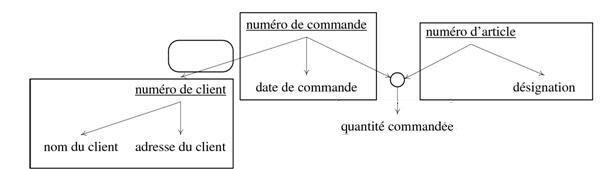
\includegraphics[width=0.9\linewidth]{graphe_identifie_3.jpg}
  \end{center}
  \begin{itemize}
    \item Étape 4 : sauf si entre deux identifiants se trouvent deux dépendances élémentaires réflexives,
      auquel cas l'association binaire a deux cardinalités maximales valant $1$
  \end{itemize}
\end{frame}

\begin{frame}
  \frametitle{Étapes de traduction (5)}
  \begin{center}
    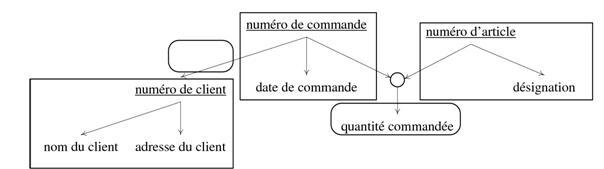
\includegraphics[width=0.9\linewidth]{graphe_identifie_5.jpg}
  \end{center}
  \begin{itemize}
    \item Étape 5 : les attributs (non identifiants) qui dépendent de plusieurs identifiants sont les
      attributs d'une association supplémentaire dont les cardinalités maximales sont toutes $n$
  \end{itemize}
\end{frame}

\begin{frame}
  \frametitle{Schéma obtenu}
  \begin{center}
    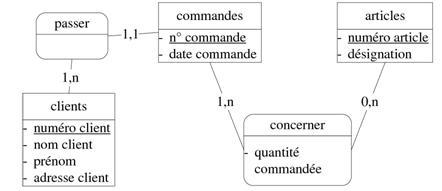
\includegraphics[width=0.9\linewidth]{schema_traduit.jpg}
  \end{center}
\end{frame}

\begin{frame}
  \frametitle{Remarques}
  \begin{itemize}
    \item Il faut donner un nom aux entités et aux associations
    \item Il reste les cardinalités minimales à établir
    \item En pratique, il faut connaître les entités pour établir le graphe de couverture minimale
    \item[$\ra$] Aide surtout à:
      \begin{itemize}
        \item Établir les associations entre les entités
        \item Normaliser les entités et leurs associations jusqu'en troisième forme normale de Boyce-Codd 
      \end{itemize}
  \end{itemize}
\end{frame}

\begin{frame}
  \frametitle{Méthodologie avec dépendances fonctionnelles}
  \begin{itemize}
    \item Identifier les entités et leur donner un identifiant
    \item Ajouter les attributs et leur dépendances fonctionnelles directes avec les identifiants
      (commencer par les dépendances élémentaires)
    \item Traduire le graphe de couverture minimale obtenu en un schéma entités-associations
    \item Ajuster les cardinalités minimales
    \item La majorité des règles de normalisation devraient être vérifiées, vérifier notamment:
      \begin{itemize}
        \item La normalisation des noms
        \item Les attributs en plusieurs exemplaires
        \item Les associations redondantes ou en plusieurs exemplaires
      \end{itemize}
  \end{itemize}
\end{frame}

% \begin{frame}
%   \frametitle{Remarques}
%   \begin{itemize}
%     \item Le modèle doit :
%       \begin{itemize}
%         \item Être \emph{exhaustif} : contenir toutes les informations nécessaires
%         \item Éviter les \emph{redondances} : perte d'espace, plus de travail de maintenance, risque d'incohérence
%       \end{itemize}
%     \item Ces méthodologies sont plutôt utilisées itérativement pour converger vers une modélisation
%       pertinente
%   \end{itemize}
% \end{frame}

%\subsection{Cas particuliers}
\begin{frame}
  \frametitle{Gestion des dates et de l'historique (1)}
  \begin{itemize}
    \item Dans une bibliothèque, on peut vouloir stocker les emprunts en cours ou les emprunts historiques
  \end{itemize}
  \begin{center}
    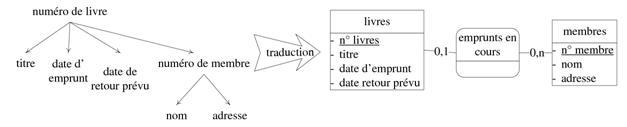
\includegraphics[width=0.9\linewidth]{emprunts_en_cours.jpg}
  \end{center}
  \begin{itemize}
    \item Emprunts en cours : la date de retour prévu est un attribut de l'entité livres car un livre
      ne peut faire l'objet que d'un seul emprunt en cours
  \end{itemize}
\end{frame}

\begin{frame}
  \frametitle{Gestion des dates et de l'historique (2)}
  \begin{itemize}
    \item Emprunts historiques :
      \begin{itemize}
        \item Un livre peut faire l'objet de plusieurs emprunts historiques
        \item Date d'emprunt est nécessaire pour connaître la date de retour prévue
        \item On évite d'avoir une date comme identifiant
        \item Une dépendance fonctionnelle ne peut partir que d'un ou plusieurs identifiant(s)
      \end{itemize}
    \item[$\ra$] C'est le signe qu'il manque un identifiant : le numéro d'emprunt
  \end{itemize}
\end{frame}

\begin{frame}
  \frametitle{Gestion des dates et de l'historique (3)}
  \begin{center}
    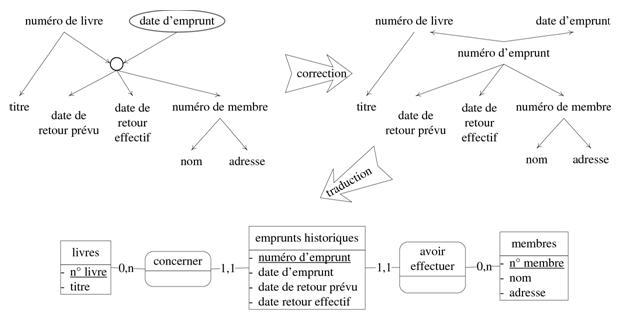
\includegraphics[width=0.9\linewidth]{gestion_historique.jpg}
  \end{center}
\end{frame}

\begin{frame}
  \frametitle{Gestion des dates et de l'historique (4)}
  \begin{itemize}
    \item Même pour une entité historisée, il vaut mieux éviter que la date n'entre dans l'identifiant
    \item Ici, l'entité emprunts historiques ne peut pas être transformée en une association (normalisation
      des attributs des associations) :\\ date retour effectif ne dépend pas du numéro de livre et du numéro de membre, mais du numéro de livre et de la date
      d'emprunt
    % \item La normalisation des entités ne s'applique donc pas aux entités qui ont un caractère historique
    \item[$\ra$] Si il n'y avait que le numéro et la date d'emprunt, on pourrait
        utiliser une association
  \end{itemize}
\end{frame}

\begin{frame}
  \frametitle{Dépendances plurielles}
  \begin{itemize}
    \item Une ou plusieurs dépendances fonctionnelles partent ou arrivent plusieurs fois du même
      attribut
  \end{itemize}
  \begin{center}
    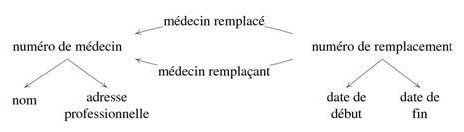
\includegraphics[width=0.9\linewidth]{dependances_plurielles.jpg}
  \end{center}
  \begin{itemize}
    \item Ajouter un commentaire sur la flèche permet de clarifier la signification de chaque dépendance
    \item Ce commentaire donnera le nom des associations correspondantes
    \item Dépendances fonctionnelles entre médecins et remplacements\\$\ra$ associations plurielles entre entités médecins et remplacements
  \end{itemize}
\end{frame}

\begin{frame}
  \frametitle{Dépendances réflexives}
  \begin{itemize}
    \item Dépendances fonctionnelles réflexives : $X \ra X$
  \end{itemize}
  \begin{center}
    
\includegraphics[width=0.9\linewidth]{dependances_reflexives.jpg}
  \end{center}
  \begin{itemize}
    \item Intérêt : seulement si elles ont une signification particulière
  \end{itemize}
\end{frame}

\begin{frame}
  \frametitle{Associations sans attributs}
  \begin{itemize}
    \item Attention : associations avec cardinalités maximales $n$ et sans attribut ne figurent pas sur le
      graphe de couverture minimale
  \end{itemize}
  \begin{center}
    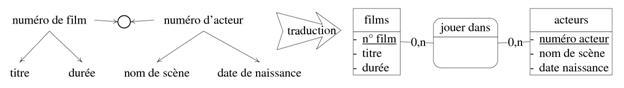
\includegraphics[width=\linewidth]{association_sans_attribut.jpg}
  \end{center}
  \begin{itemize}
    \item Possiblilité d'introduire une notation spéciale
    \item Exemple: une dépendance non élémentaire qui ne débouche sur aucun attribut
  \end{itemize}
\end{frame}
